% =============================================================================
% preamble.tex
% All package imports, styling, custom commands, listings settings, and
% bibliography configuration for the ANN Accelerator Controller report.
% =============================================================================

% --- Page geometry --------------------------------------------------------
\usepackage[a4paper,margin=2.7cm,headheight=15pt]{geometry}

% --- Core typography / micro-typography ----------------------------------
\usepackage[T1]{fontenc}
\usepackage[utf8]{inputenc}
\usepackage{lmodern}
\usepackage{microtype}
\usepackage{csquotes}

% --- Math -----------------------------------------------------------------
\usepackage{amsmath}
\usepackage{amssymb}
\usepackage{siunitx}

% --- Tables ---------------------------------------------------------------
\usepackage{booktabs}
\usepackage{tabularx}
\usepackage{longtable}
\usepackage{array}
\usepackage{multirow}

% --- Graphics and floats --------------------------------------------------
\usepackage{graphicx}
\graphicspath{{figures/}}
\usepackage{float}
\usepackage{caption}
\usepackage{subcaption}

% --- Graceful handling of missing figures --------------------------------
% Render a labelled placeholder instead of aborting the build when a
% referenced figure file is not on disk yet (e.g. a diagram that has
% not yet been exported). Compilation proceeds end-to-end and the
% placeholder makes the gap visible in the PDF.
\makeatletter
\newcommand{\GfxPlaceholder}[1]{%
  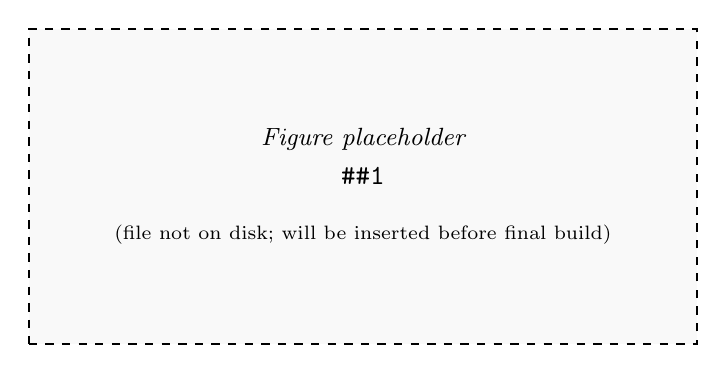
\begin{tikzpicture}
    \node[draw,thick,dashed,minimum width=0.7\linewidth,minimum height=4cm,
          align=center,fill=gray!5,inner sep=8pt]
      {\itshape\small Figure placeholder\\[2pt]\texttt{\detokenize{#1}}\\[8pt]
       \scriptsize(file not on disk; will be inserted before final build)};
  \end{tikzpicture}%
}
\let\@orig@includegraphics\includegraphics
\renewcommand{\includegraphics}[2][]{%
  \IfFileExists{figures/#2}%
    {\@orig@includegraphics[#1]{#2}}%
    {\IfFileExists{#2}%
       {\@orig@includegraphics[#1]{#2}}%
       {\GfxPlaceholder{#2}}}%
}
\makeatother

% --- Colors ---------------------------------------------------------------
\usepackage{xcolor}
\definecolor{codebg}{RGB}{248,248,248}
\definecolor{codeframe}{RGB}{210,210,210}
\definecolor{codekw}{RGB}{0,0,150}
\definecolor{codetype}{RGB}{128,0,128}
\definecolor{codecomment}{RGB}{80,120,80}
\definecolor{codestring}{RGB}{170,40,40}
\definecolor{codenumber}{RGB}{120,120,120}

% --- Lists / enumerations -------------------------------------------------
\usepackage{enumitem}
\setlist{topsep=2pt,itemsep=2pt,parsep=0pt}

% --- TikZ (available for inline diagrams if needed) ----------------------
\usepackage{tikz}
\usetikzlibrary{arrows.meta,positioning,shapes.geometric,calc,fit,backgrounds}

% --- Section titling ------------------------------------------------------
\usepackage{titlesec}
\titleformat{\chapter}[display]
  {\normalfont\Huge\bfseries}{\chaptertitlename\ \thechapter}{20pt}{\Huge}
\titlespacing*{\chapter}{0pt}{-20pt}{30pt}

% --- Headers and footers --------------------------------------------------
\usepackage{fancyhdr}
\pagestyle{fancy}
\fancyhf{}
\renewcommand{\chaptermark}[1]{\markboth{\thechapter.\ #1}{}}
\renewcommand{\sectionmark}[1]{\markright{\thesection.\ #1}}
\fancyhead[L]{\small\leftmark}
\fancyhead[R]{\small\thepage}
\renewcommand{\headrulewidth}{0.3pt}

% --- Hyperlinks and cross-references -------------------------------------
\usepackage[colorlinks=true,
            linkcolor=black,
            citecolor=black,
            urlcolor=blue!60!black,
            pdfborder={0 0 0}]{hyperref}
\usepackage[capitalise,noabbrev]{cleveref}

% --- Listings (SystemVerilog + plain) -------------------------------------
\usepackage{listings}

\lstdefinelanguage{SystemVerilog}{
  morekeywords={
    module, endmodule, input, output, inout, wire, reg, logic,
    always, always_ff, always_comb, always_latch, posedge, negedge,
    if, else, case, endcase, unique, priority, default,
    begin, end, parameter, localparam, typedef, enum, package, endpackage,
    import, export, function, endfunction, task, endtask, return,
    for, while, do, foreach, break, continue,
    assign, initial, final, generate, endgenerate, genvar,
    interface, endinterface, modport, virtual, class, endclass, new,
    extends, implements, super, this, pure, ref, const,
    bit, byte, shortint, int, longint, integer, real, time, shortreal,
    string, chandle, event, void,
    signed, unsigned, packed, struct, union,
    automatic, static, rand, randc, constraint
  },
  keywordstyle=\color{codekw}\bfseries,
  morekeywords=[2]{localparam,typedef,enum,struct},
  keywordstyle=[2]\color{codetype}\bfseries,
  morecomment=[l]{//},
  morecomment=[s]{/*}{*/},
  commentstyle=\color{codecomment}\itshape,
  morestring=[b]",
  stringstyle=\color{codestring},
  sensitive=true,
  alsoletter={\_},
}

\lstdefinestyle{svstyle}{
  language=SystemVerilog,
  backgroundcolor=\color{codebg},
  basicstyle=\ttfamily\footnotesize,
  numbers=left,
  numberstyle=\tiny\color{codenumber},
  numbersep=6pt,
  frame=single,
  rulecolor=\color{codeframe},
  framesep=4pt,
  xleftmargin=16pt,
  tabsize=2,
  showstringspaces=false,
  breaklines=true,
  breakatwhitespace=true,
  captionpos=b,
  aboveskip=10pt,
  belowskip=6pt,
}

\lstdefinestyle{plainstyle}{
  backgroundcolor=\color{codebg},
  basicstyle=\ttfamily\footnotesize,
  numbers=none,
  frame=single,
  rulecolor=\color{codeframe},
  framesep=4pt,
  xleftmargin=8pt,
  tabsize=2,
  showstringspaces=false,
  breaklines=true,
  breakatwhitespace=true,
  captionpos=b,
  aboveskip=10pt,
  belowskip=6pt,
}

\lstset{style=svstyle}

% --- Custom commands ------------------------------------------------------
\newcommand{\sv}[1]{\texttt{#1}}
\newcommand{\modname}[1]{\texttt{#1}}
\newcommand{\signame}[1]{\texttt{#1}}
\newcommand{\stateval}[1]{\texttt{#1}}

% --- Bibliography (biblatex + biber) -------------------------------------
\usepackage[backend=biber,
            style=numeric-comp,
            sorting=none,
            maxbibnames=99]{biblatex}
\addbibresource{references.bib}

% --- Table of contents depth ---------------------------------------------
\setcounter{tocdepth}{2}
\setcounter{secnumdepth}{3}
